\chapter{System Testing and Verification}
\label{ch:system-testing}

This chapter introduces you to the testing setup and how we tested each module in isolation and the end-to-end integration that we planned and followed to prove to a high certainty the correctness of the system.

Testing ad-hoc networks always has been very tricky subjects, with researchers spending big amounts of funds on building testbeds with actual hardware and workers who move the hardware/devices around to change the connectivity between them.
It is a tedious task to test ad-hoc protocols on actual hardware.
The problem is harder when you want to execute the test multiple times.
It is very costly in terms of money and time and other resources.

This is why we took the decision, which some researchers take, and aimed to emulate the environment the system would likely be deployed on.
Most researchers take the path of network simulation, the difference is that with simulation, results are less accurate because of time compression and the lack of real world constrains like power consumption and latency while communicating with the kernel.
With emulation, we can run the protocol implementation in real time while integrating it with real kernel.
This enables us to explore how routing solutions could be built and constructed for real world systems, and let us face real world challenges regarding routing implementation.
Also, with emulation, we can run real applications on top of the router to test its performance.

Nevertheless, emulation lacks the capability of spawning big number of nodes due to the limits of computer's memory and because each node is an entire VM/container with real programs.
Kernel scheduler and memory management put limitations on the number of nodes' wireless devices we can emulate.

The next sections will walk you through our setup, scripts, GUIs and plans to prove the correctness of the programs we built in \acrshort{caian}.

\section{Testing Setup}
\subsection{Mininet-Wifi}
Mininet-Wifi is a python program and library that emulates wireless networks in infrastructure and ad-hoc modes.
It's a wrapper around Mininet project, which aims to emulate software defined networks for research and education.
It relies on \textit{wmediumd} and \textit{mac80211\_hwsim} kernel modules to simulate wireless radio devices and uses network namespaces feature from Linux to isolate processes as if they are in their own device.

With \textit{wmediumd}, Mininet-Wifi can simulate the propagation of wireless signals and control the probabilities of dropping packets and adding noise to them. 

Figure \ref{fig:mininet-diagram} shows unit and command nodes running inside a testbed created by Mininet, each node should have a router process.

\begin{figure}
    \centering
    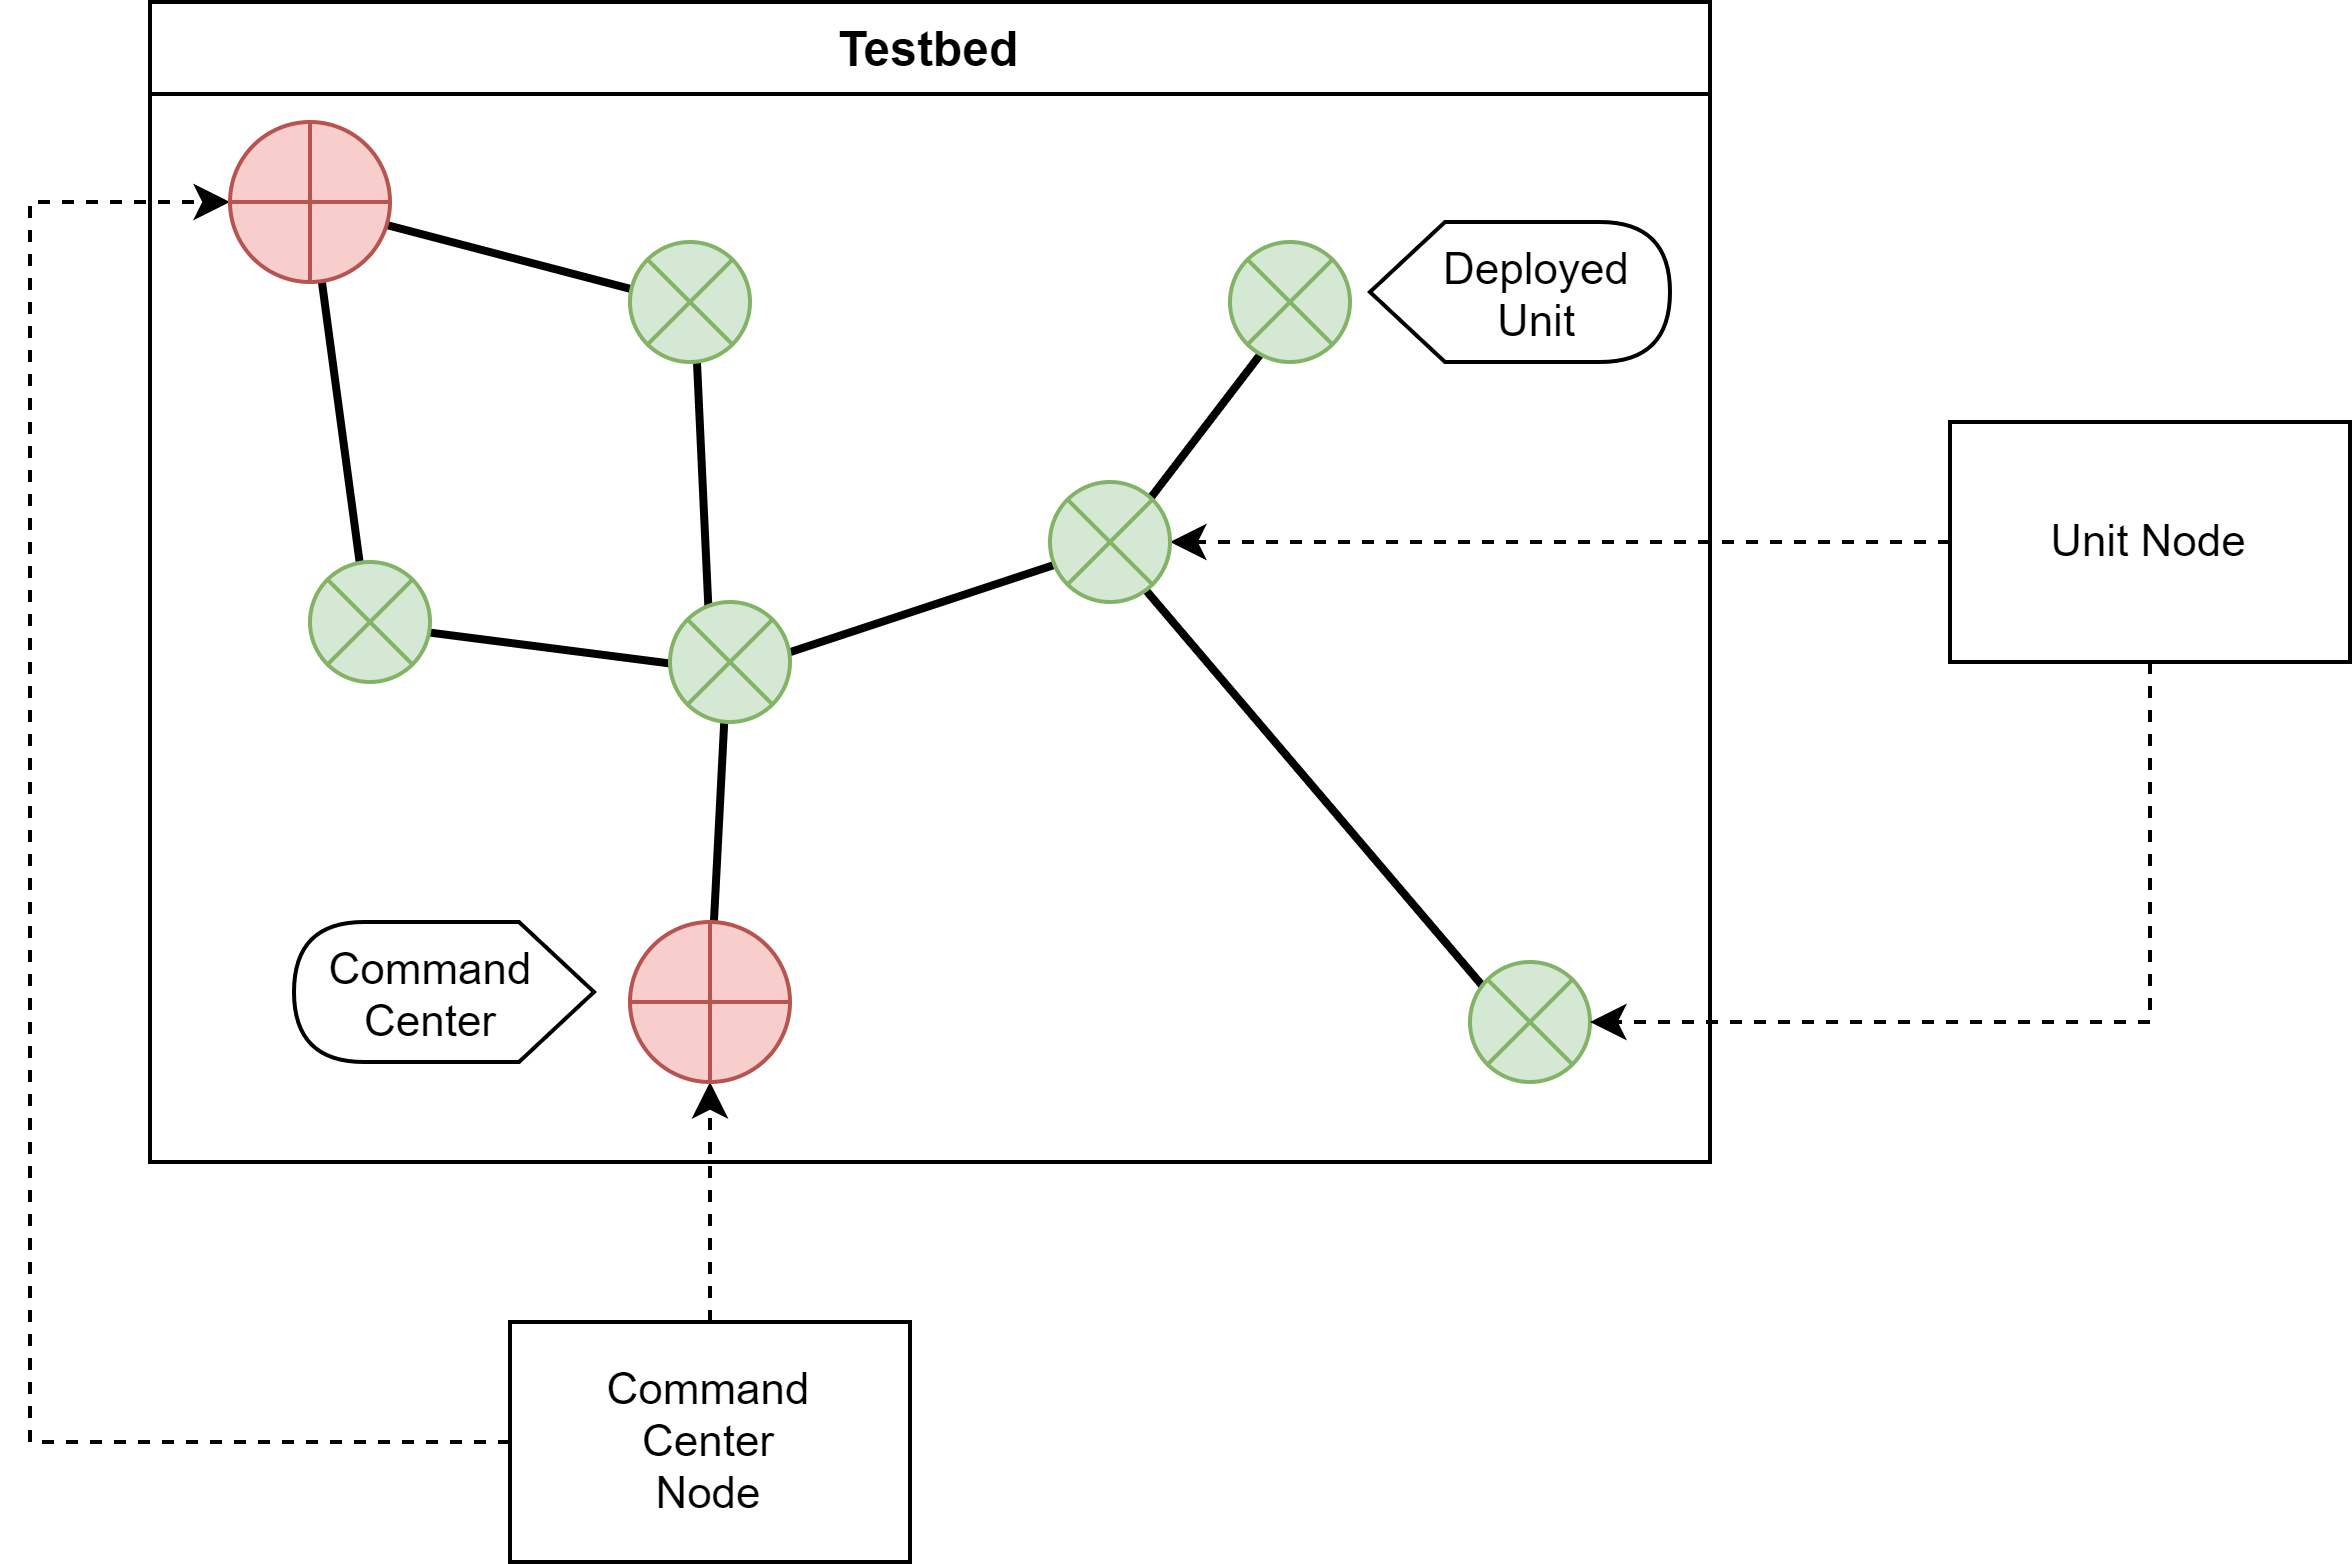
\includegraphics[width=13cm]{images/nodes_diagram.png}
    \caption{Mininet Testbed With Different Nodes}
    \label{fig:mininet-diagram}
\end{figure}

\subsubsection{Installing Mininet-Wifi}
Run the following:
\begin{verbatim}
$ python --version
\end{verbatim}

If it's 3, you are good to go, otherwise do the following:

\begin{verbatim}
$ sudo mv /bin/python /bin/python.old
$ sudo ln /bin/python3 /bin/python
\end{verbatim}

It may break your system, in this case reverse it back: 
\begin{verbatim}
sudo m /bin/python.old /bin/python
\end{verbatim}

Then install mininet-wifi:

\begin{verbatim}
$ (
    set -e
    sudo apt update
    sudo apt install -y git
    cd /tmp
    git clone git://github.com/intrig-unicamp/mininet-wifi
    sudo mininet-wifi/util/install.sh -Wln
)   
\end{verbatim}

\subsection{Edit GUI and MN Script}
To be able to create, edit and visualize the topology either offline or online (while Mininet-Wifi is running), we created \textit{edit} which is a web GUI for the testbed. 

Figure \ref{fig:edit-ui} shows edit UI, it has a map with units each has its name and range, you can move/add/delete nodes and change the hierarchical zones \textit{Zlen} and apply a mobility simulation with some configuration while connected to Mininet.

\begin{figure}[!htbp]
    \centering
    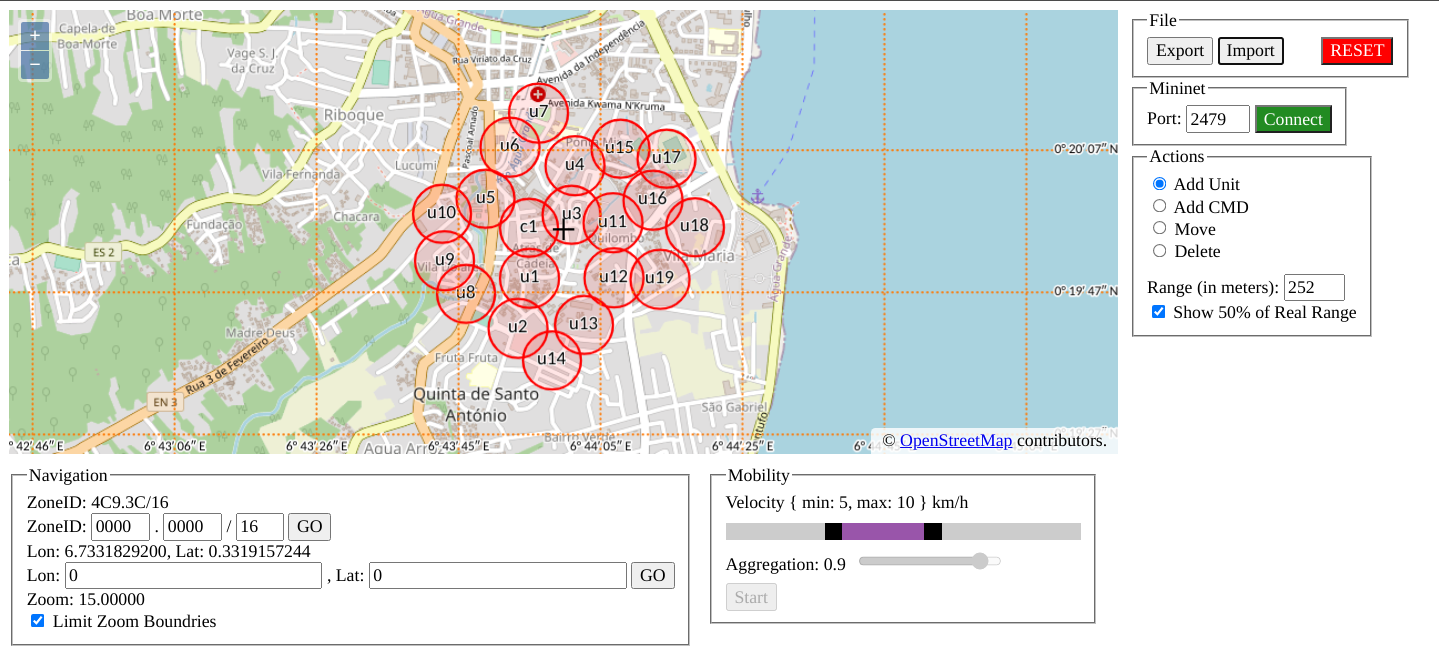
\includegraphics[width=15cm]{images/edit-ui.png}
    \caption{Edit GUI}
    \label{fig:edit-ui}
\end{figure}

Edit can export and import the topology into a specific format we made for the testbed.
Also edit can connect to a script we wrote that controls the routers and units and Mininet, edit gets updates about nodes' locations in case the script is moving them (while in mobility mode) or edit sends location updates in case the user is moving the nodes manually.

The script - called mn, written in python - uses a modified copy of pymobility which implements ``Time Variant Community'' Mobility or TVC for short, which works by defining a group of units and the model keeps them around some moving center it calculates.
This mobility model resembles the soldiers' units moving around, because most probably they won't walk randomly in different directions, but rather in groups together.

With ``aggregation'' control switch, you can in edit specify how much the group should move together, where 0 aggregation means every node is on its own.

The mn script sends the locations (longitude and latitude) for each node periodically through Unix sockets open by routers and units on the nodes.

\subsection{Start Script}
Start is a script that can any component of the system, whether it's on the localhost or inside the Mininet namespaces.
The following is how to run Mininet on some topology and routers and units and command centers' daemons and \acrshort{hal}s using start:
\begin{verbatim}
## (1st terminal)
# start mininet-wifi within chromosome topology
$ sudo ./start mn topos/chromosome.topo

## (2nd terminal)
# start routers in all nodes
$ sudo ./start routers

## (3rd terminal)
$ sudo ./start units
## (4th terminal)
$ sudo ./start cmds
## (5th terminal)
$ sudo ./start hals
\end{verbatim}

Start lists Mininet namespaces using pgrep, then injects programs into the Mininet containers using nsenter and watches for file changes using watchdog script.

\subsubsection{Socat}

The CMD UI and Unit UI can only communicate with their daemons using TCP sockets, but the daemons are isolated in the namespaces and running any GUI inside is tedious and maybe impossible (due to X11/Wayland using TCP sockets and residing outside the namespace) this is why we used \textit{socat} utility to forward TCP sockets in the host machine to Unix sockets that are exposed by the daemons.
Because Unix sockets are [virtual] files, and the namespaces are just network namespaces, the Unix sockets are not isolated inside the namespaces, so we could forward them into TCP sockets for the UI.
This helped us avoid changing the interface for the UI just to test inside the testbed.

Figure \ref{fig:socat-diagram} shows how the socket forwarding happens with the testbed.

\begin{figure}[!htbp]
    \centering
    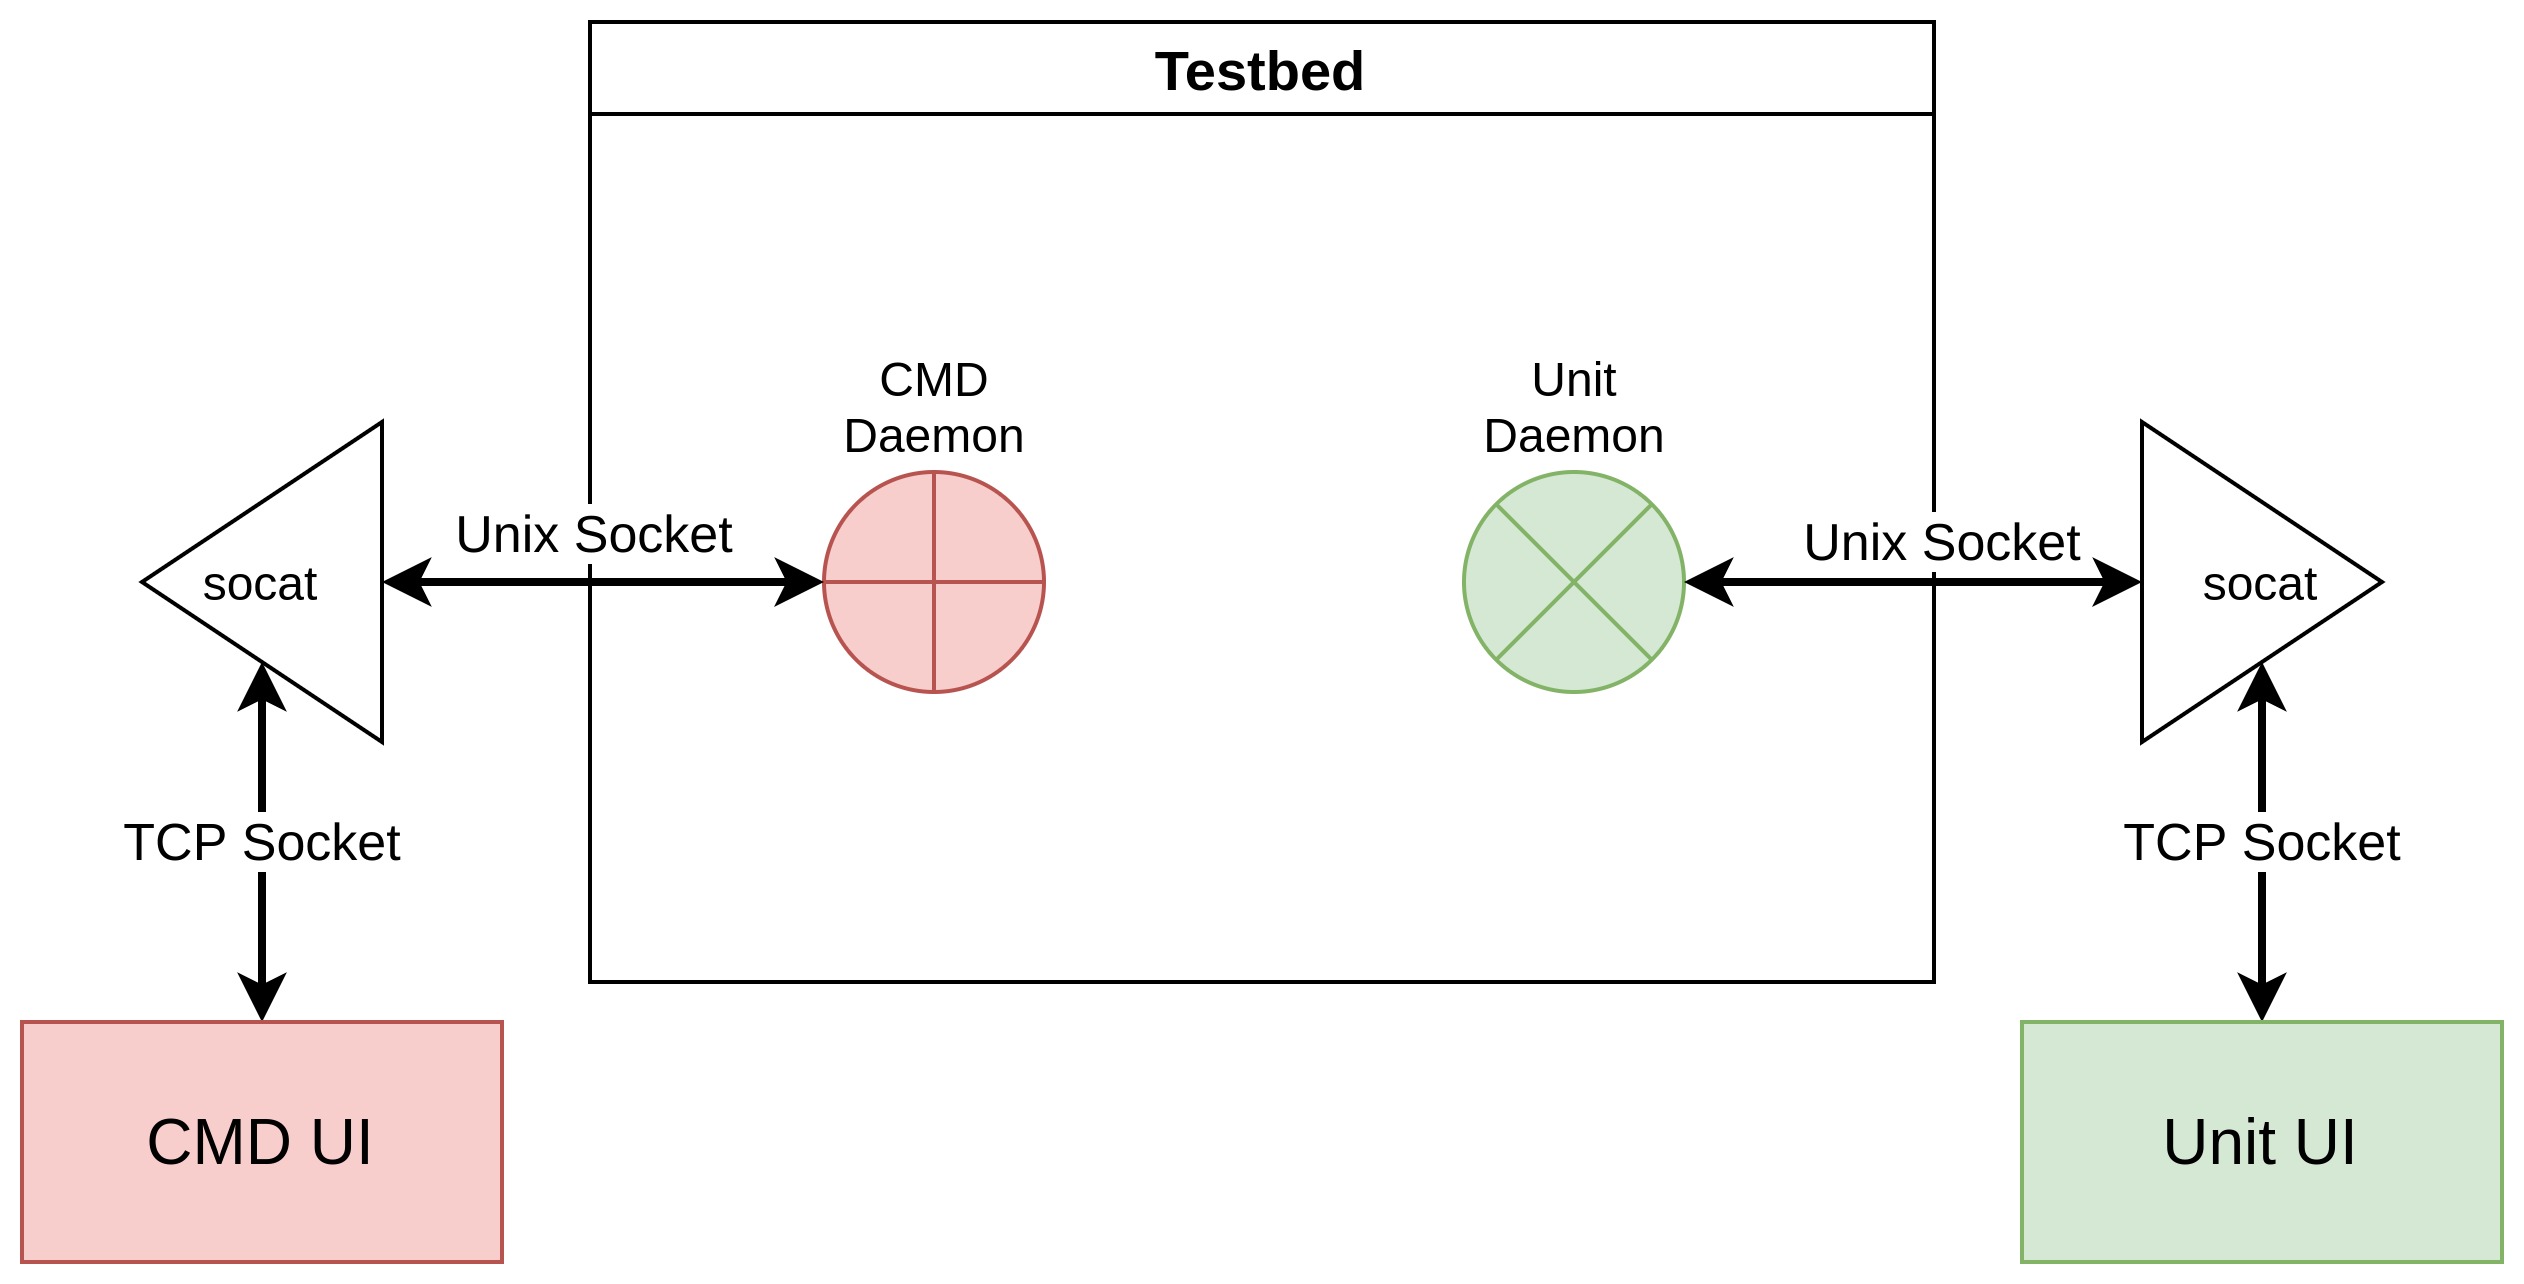
\includegraphics[width=13cm]{images/socat-diagram.png}
    \caption{Socat Forwarding and UI}
    \label{fig:socat-diagram}
\end{figure}

\section{Testing Plan and Strategy}
Our main goal in evaluating each module in \acrshort{caian} was to make sure it met all functional and non-functional requirements that were specified earlier. Testing is almost as challenging as development, if not more difficult in the world of networks, especially ad-hoc networks. We were very cautious from the very beginning of this project to provide a testing environment that allowed us to test each and every stage of the development process. For example, the sARP protocol was one of the first implemented protocols related to the Zone-based Hierarchical Link State (\acrshort{zhls}) unicast protocol; at this stage, we must ensure that the protocol is functioning properly, that each node can identify its neighbors, and that the delay metric to each of them is correctly measured.

For the reasons stated above, testing development could not be postponed after code development. As a result, our testing strategy was obvious from the start in terms of the need for a testing environment that allows us to construct multiple topologies with varied patterns of movement and exchange and route messages between different nodes in these topologies. \acrshort{caian} testing development plan can be mainly divided into three components as shown in Figure \ref{fig:testing-strategy}: \acrshort{utils} testing development, integration testing development and network testing development that serves both module and integration testing.

\begin{figure}[!htbp]
    \centering
    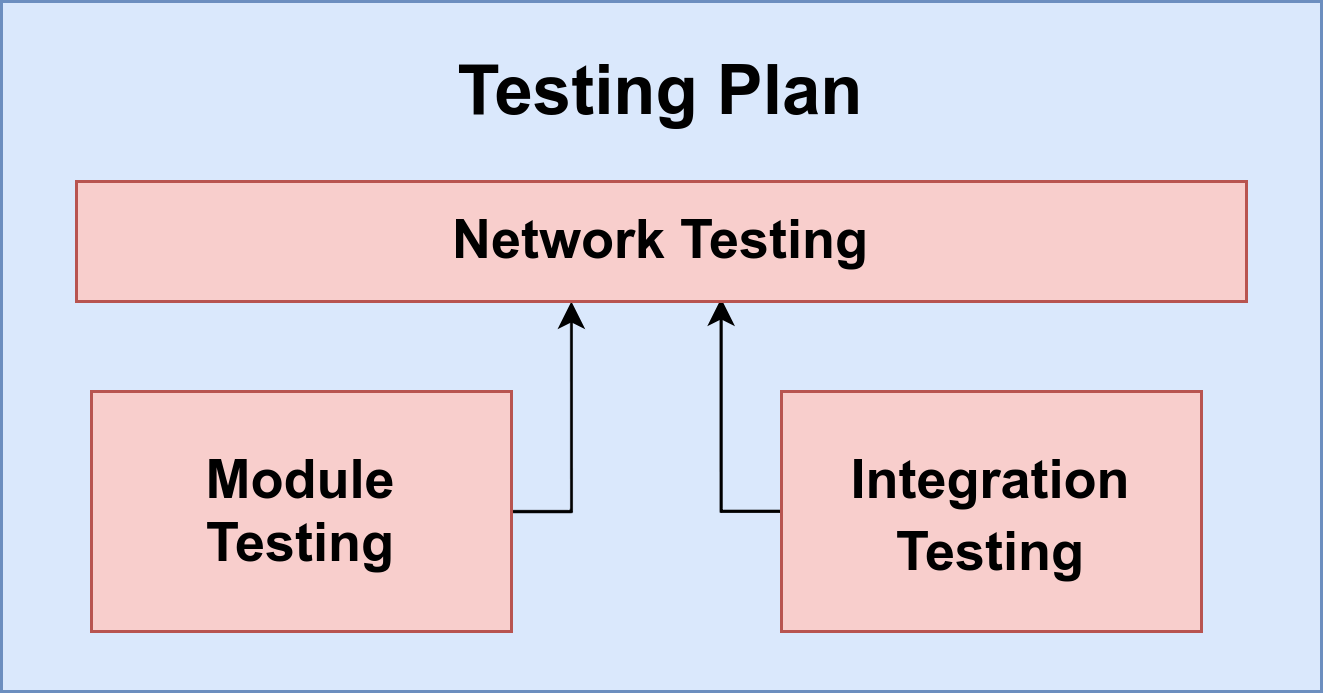
\includegraphics[width=15cm]{images/testing-plan.png}
    \caption{Testing Strategy}
    \label{fig:testing-strategy}
\end{figure}

Each component will be briefly discussed in the section below.

\subsection{Module Testing}
In \acrshort{caian}, Module testing is done sequentially into two steps as show in Figure \ref{fig:module-testing}: \acrshort{utils} testing and network testing. All protocols that need an active topology with several nodes, as well as the ability to relocate these nodes and encapsulate each in its own network namespace, fall under the network testing umbrella, and this type of testing development starts from the very beginning of our project. However, \acrshort{utils} testing was concerned with aspects that could be verified independently of the network, such as encoding, decoding, marshalling, unmarshalling, graph algorithms, tables handling, and timers. This type of testing was developed immediately after the development of its related code.

\begin{figure}
    \centering
    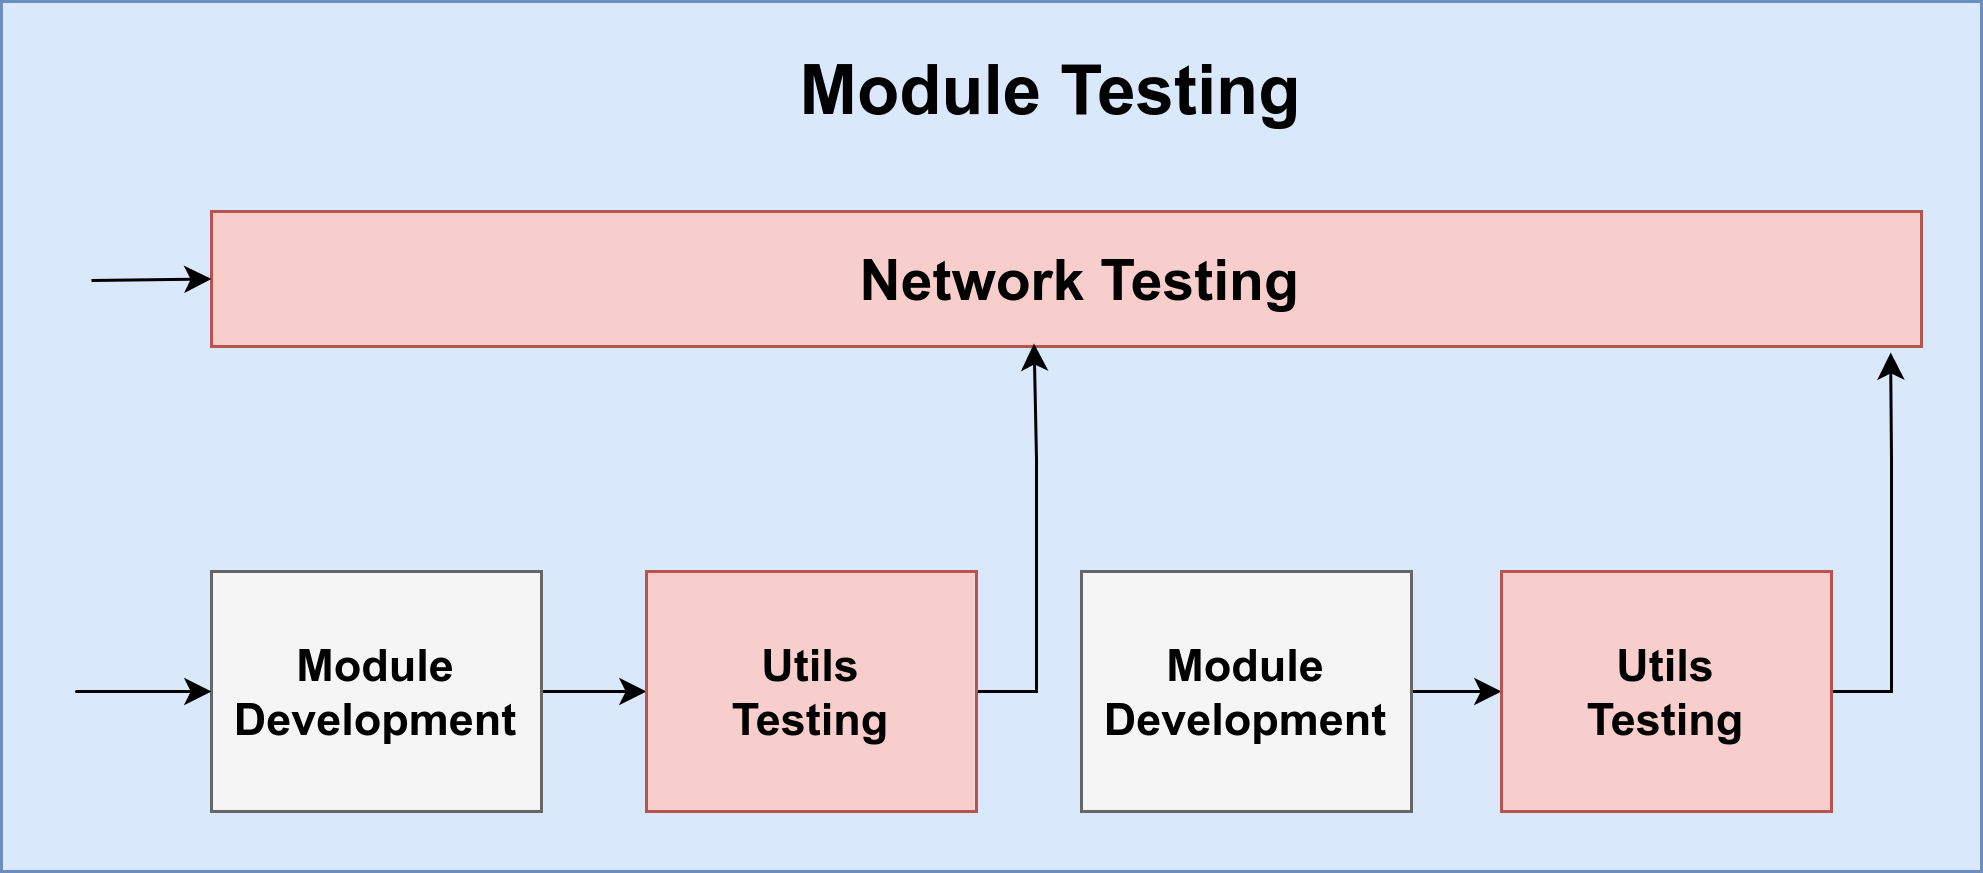
\includegraphics[width=15cm]{images/module-testing.png}
    \caption{Module Testing}
    \label{fig:module-testing}
\end{figure}


\subsection{Integration Testing}
Integration testing was a difficult process in \acrshort{caian}. It contains end-to-end testing using a topology that has numerous of nodes, each with its own user interface and router.

The integration testing was split into two primary procedures that ran simultaneously. The initial step was to evaluate the app's functionality from units to command centers and back. This process was carried out both automatically using \acrshort{hal} scripts to simulate units and send periodic sensor data and stream videos to the command center, as well as manually to test both unit and command center user interfaces and ensure that multicast and broadcast data was sent only to its intended destination.

The second step in the integration testing process was to test the routing decisions. Data delivery to its intended destination wasn't enough for us to declare that the system functioned as it's intended to be. It was critical to observe and evaluate each node's routing choice, as well as how data is delivered from its source to its intended destination. To accomplish so, we created a log visualizer software as shown in Figure \ref{fig:log-vis} that can collect all the router logs and evaluate their forwarding decisions, and displaying them to us in a way that allows us to appraise the router's performance and behavior. 

\begin{figure}[!htb]
    \centering
    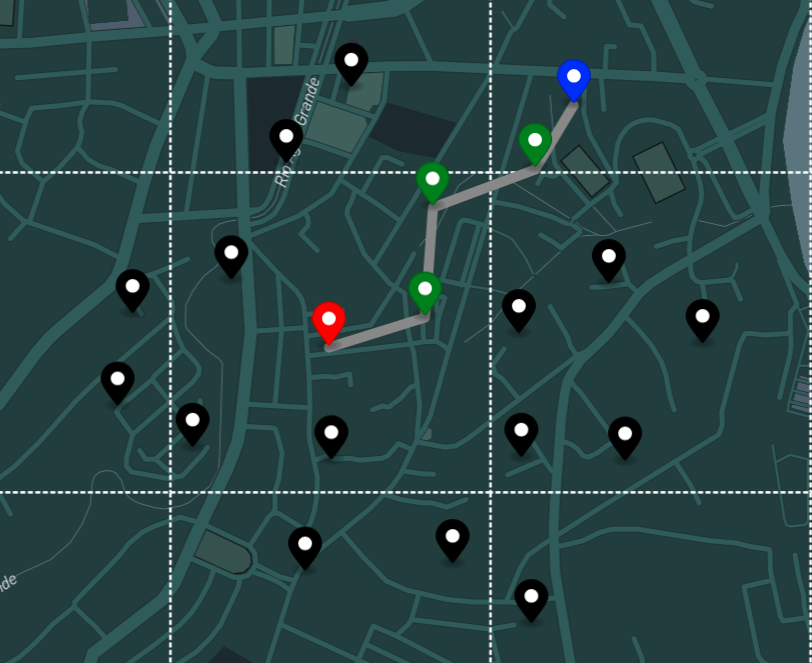
\includegraphics[width=7cm]{images/log-vis1.png}
    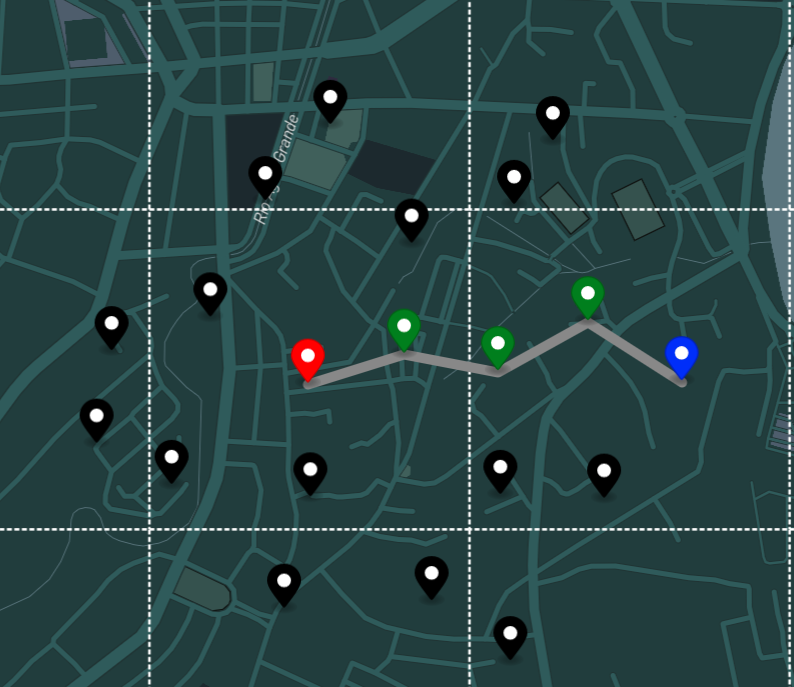
\includegraphics[trim={0 0 0 1.3cm},clip,width=7cm]{images/log-vis2.png}
    \caption{Log Visualizer}
    \label{fig:log-vis}
\end{figure}


\section{Comparative Results to Previous Work}
Table \ref{tab:comparison-table} shows the difference between our work and previous work.
We introduced new concepts and extensions to the protocols and implemented them.
All the extensions have been discussed in great detail throughout the book.

\begin{table}[!htb]
\centering
\resizebox{\textwidth}{!}{%
\begin{tabular}{|c|c|c|c|}
\hline
Protocol              & Comparison            & Previous Work           & Our Work       \\ \hline
 & Zone Size             & Constant and Predefined & Variable       \\ \cline{2-4} 
       \multirow{-2}{*}{ZHLS}               & Maintained Topologies & Two Separate            & Single Unified \\ \hline
Broadcast             & Limits                & Unbounded               & \begin{tabular}[c]{@{}c@{}}Geographically Limited \\ with a Radius\end{tabular} \\ \hline
ODMRP                 & Join Reply            & Using Flooding          & \begin{tabular}[c]{@{}c@{}}Iterating Over \\ Next Hops\end{tabular}             \\ \hline
\end{tabular}%
}
\caption{Summary of Differences Between Our Work and Previous Work}
\label{tab:comparison-table}
\end{table}

